\chapter{Il caso Unicredit - titolo provvisorio} 

La realtà in analisi è un grosso gruppo finanziario internazionale. L'ambiente
progettato e realizzato durante il mio stage aziendale elabora i
dati di circa 90000 dipendenti dell'azienda, ed è predisposto per gestirne
altrettanti aggiuntivi, alla luce di una grossa fusione avvenuta di recente.
Il sistema di gestione delle identità realizzato è subentrato gradualmente
all'architettura precedentemente esistente e, di conseguenza, la sua
progettazione ha dovuto considerare la possibilità di
inserimento graduale nel ciclo di vita di tutto il resto dell'architettura
aziendale.

Subentrare ad una realtà già esistente è stato un notevole vantaggio perchè ha
permesso di analizzare quanto già creato e migliorare i difetti più evidenti
mantenendone i punti di forza.

\section{Ambiente AS-IS}

\begin{sidewaysfigure}[tbp]
\centering
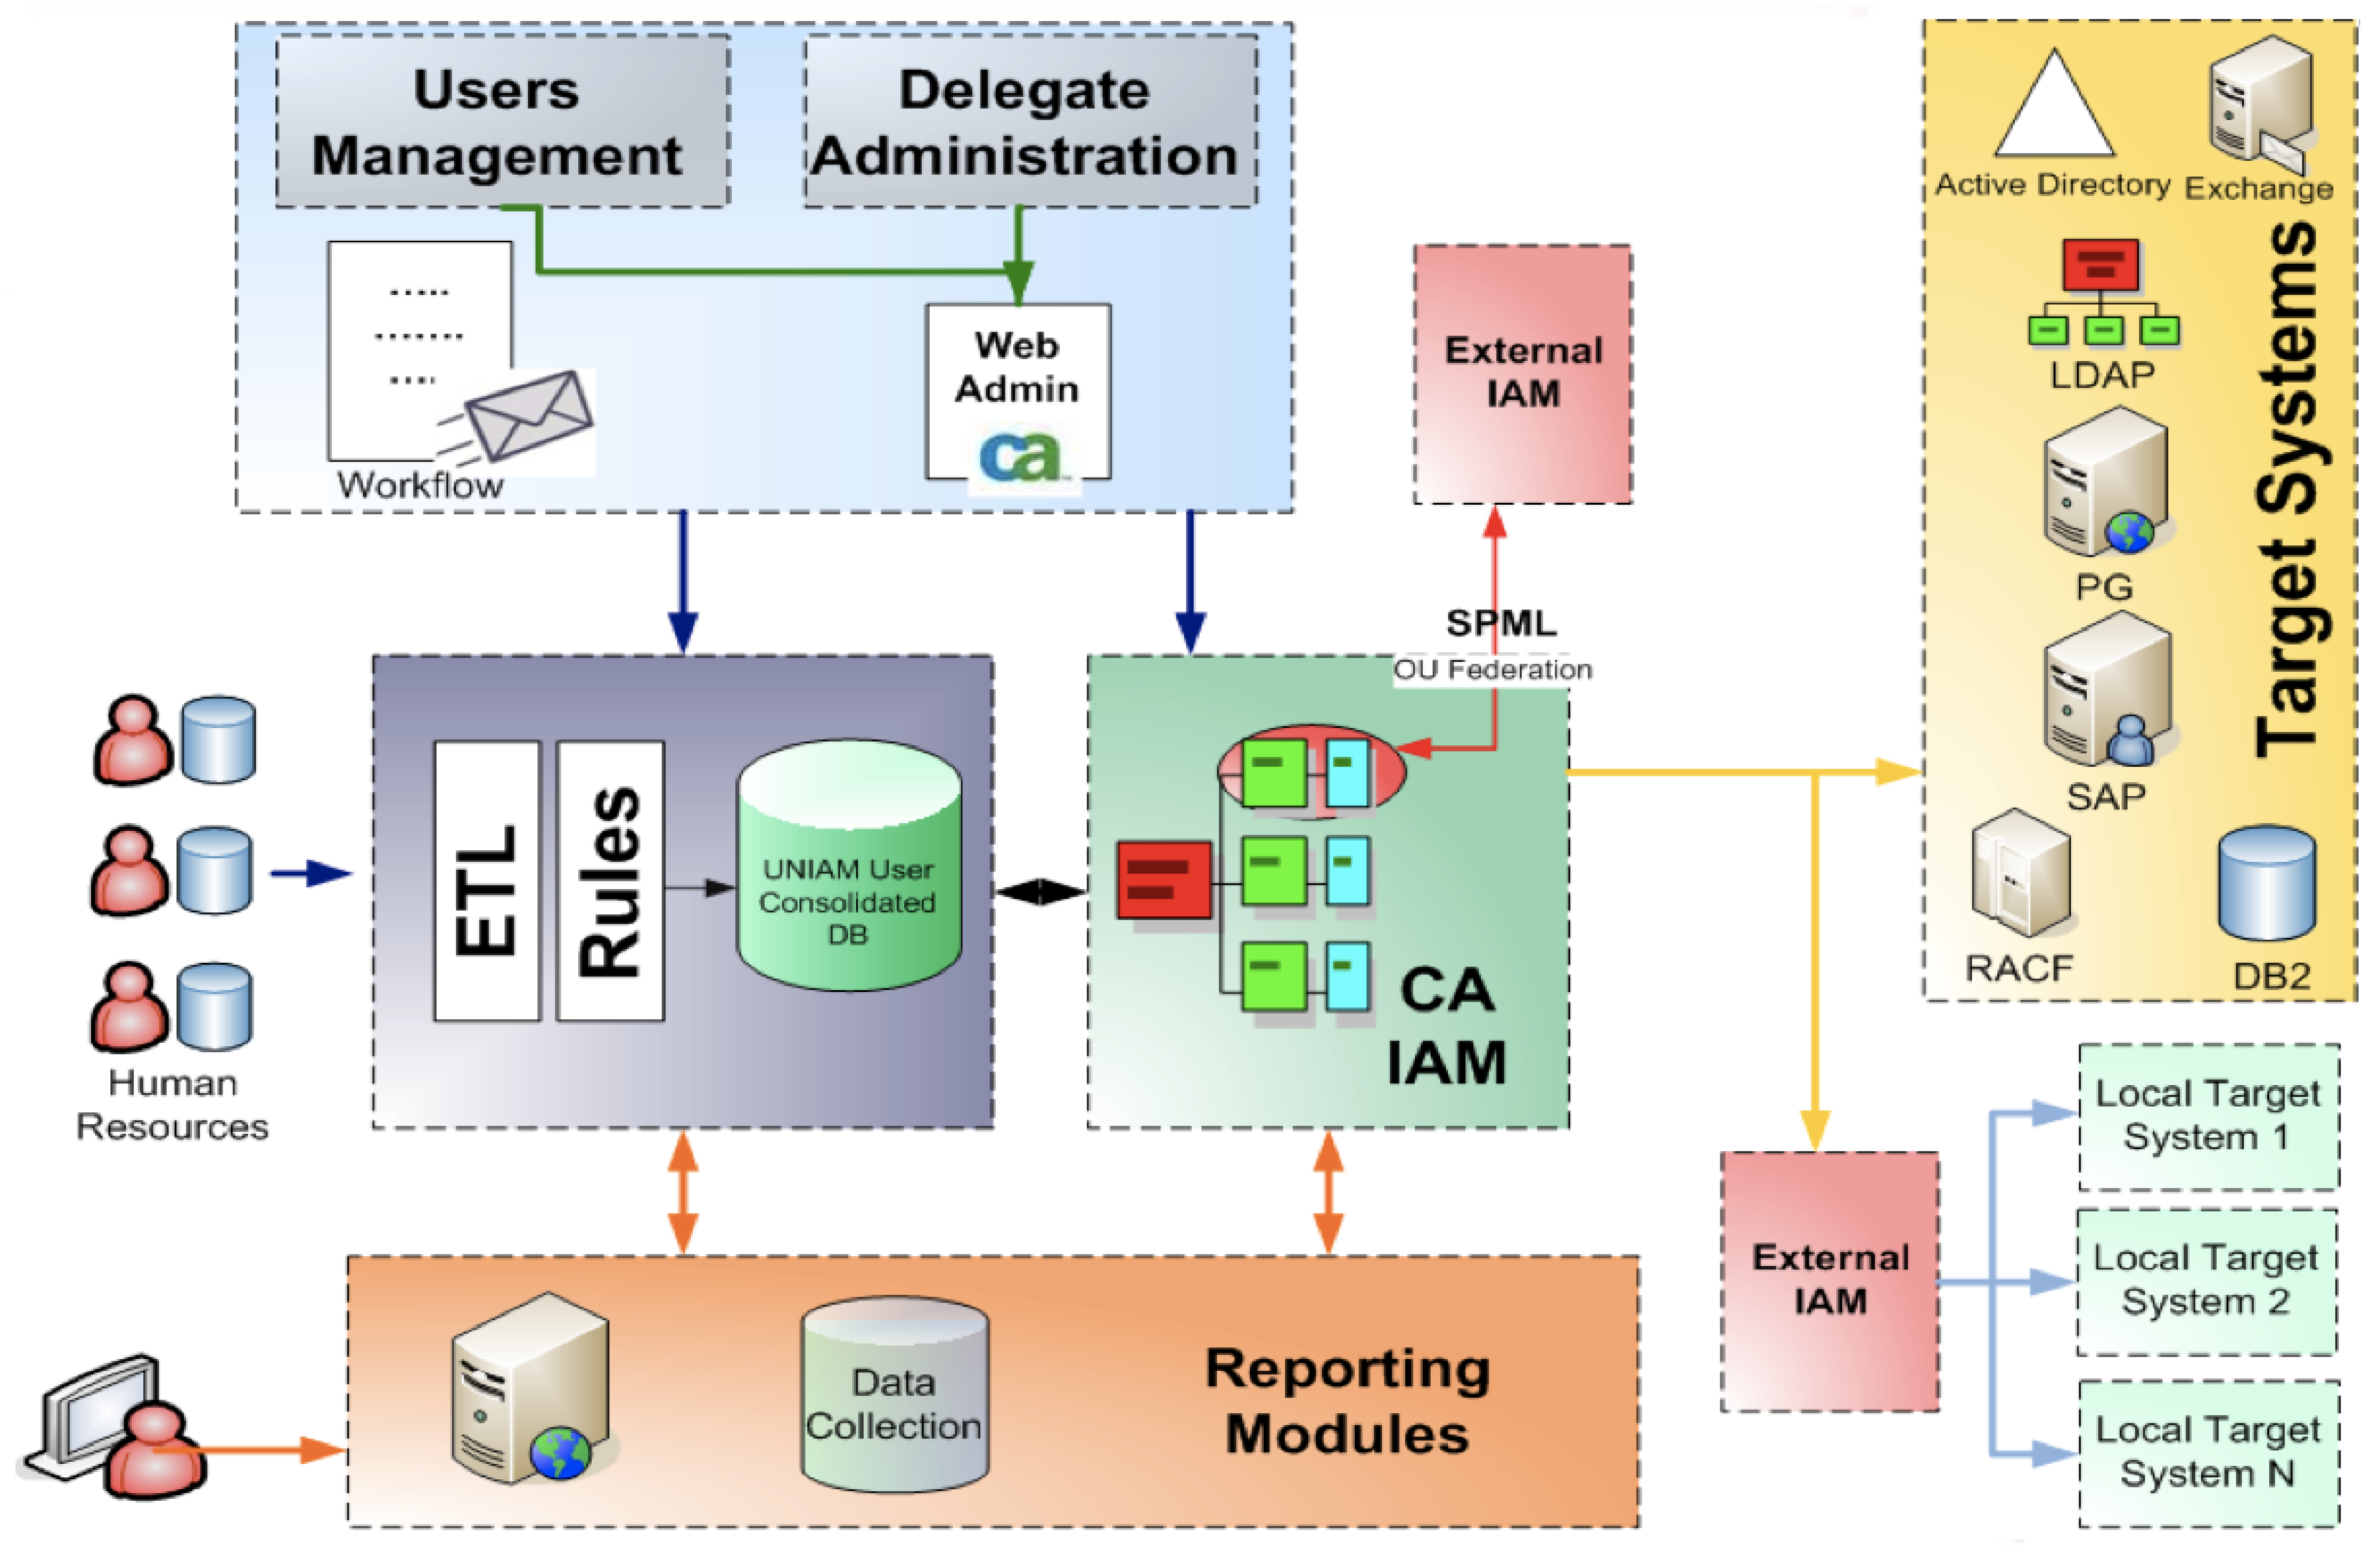
\includegraphics[width=0.95\textwidth]{img/soluzioneCA.eps}
\caption{Architettura IAM}
\label{soluzioneCA}
\end{sidewaysfigure}

In figura\ref{soluzioneCA} è illustrata la soluzione completa attualmente
funzionante. La maggior parte delle componenti di IAM presenti è implementata
con prodotti di Computer Associates~\footnote{CA - http://www.ca.com}.

Il sistema si occupa della gestione del personale di quasi tutto il gruppo
bancario. Alcune banche e assicurazioni controllate non sono state ancora
inserite, benchè la loro integrazione sia prevista entro la fine del 2009.
Un'immagine rappresentativa delle prestazioni ottenute è rappresentata in
figura~\ref{descrizioneprogetto}


\begin{sidewaysfigure}[tbp]
\centering
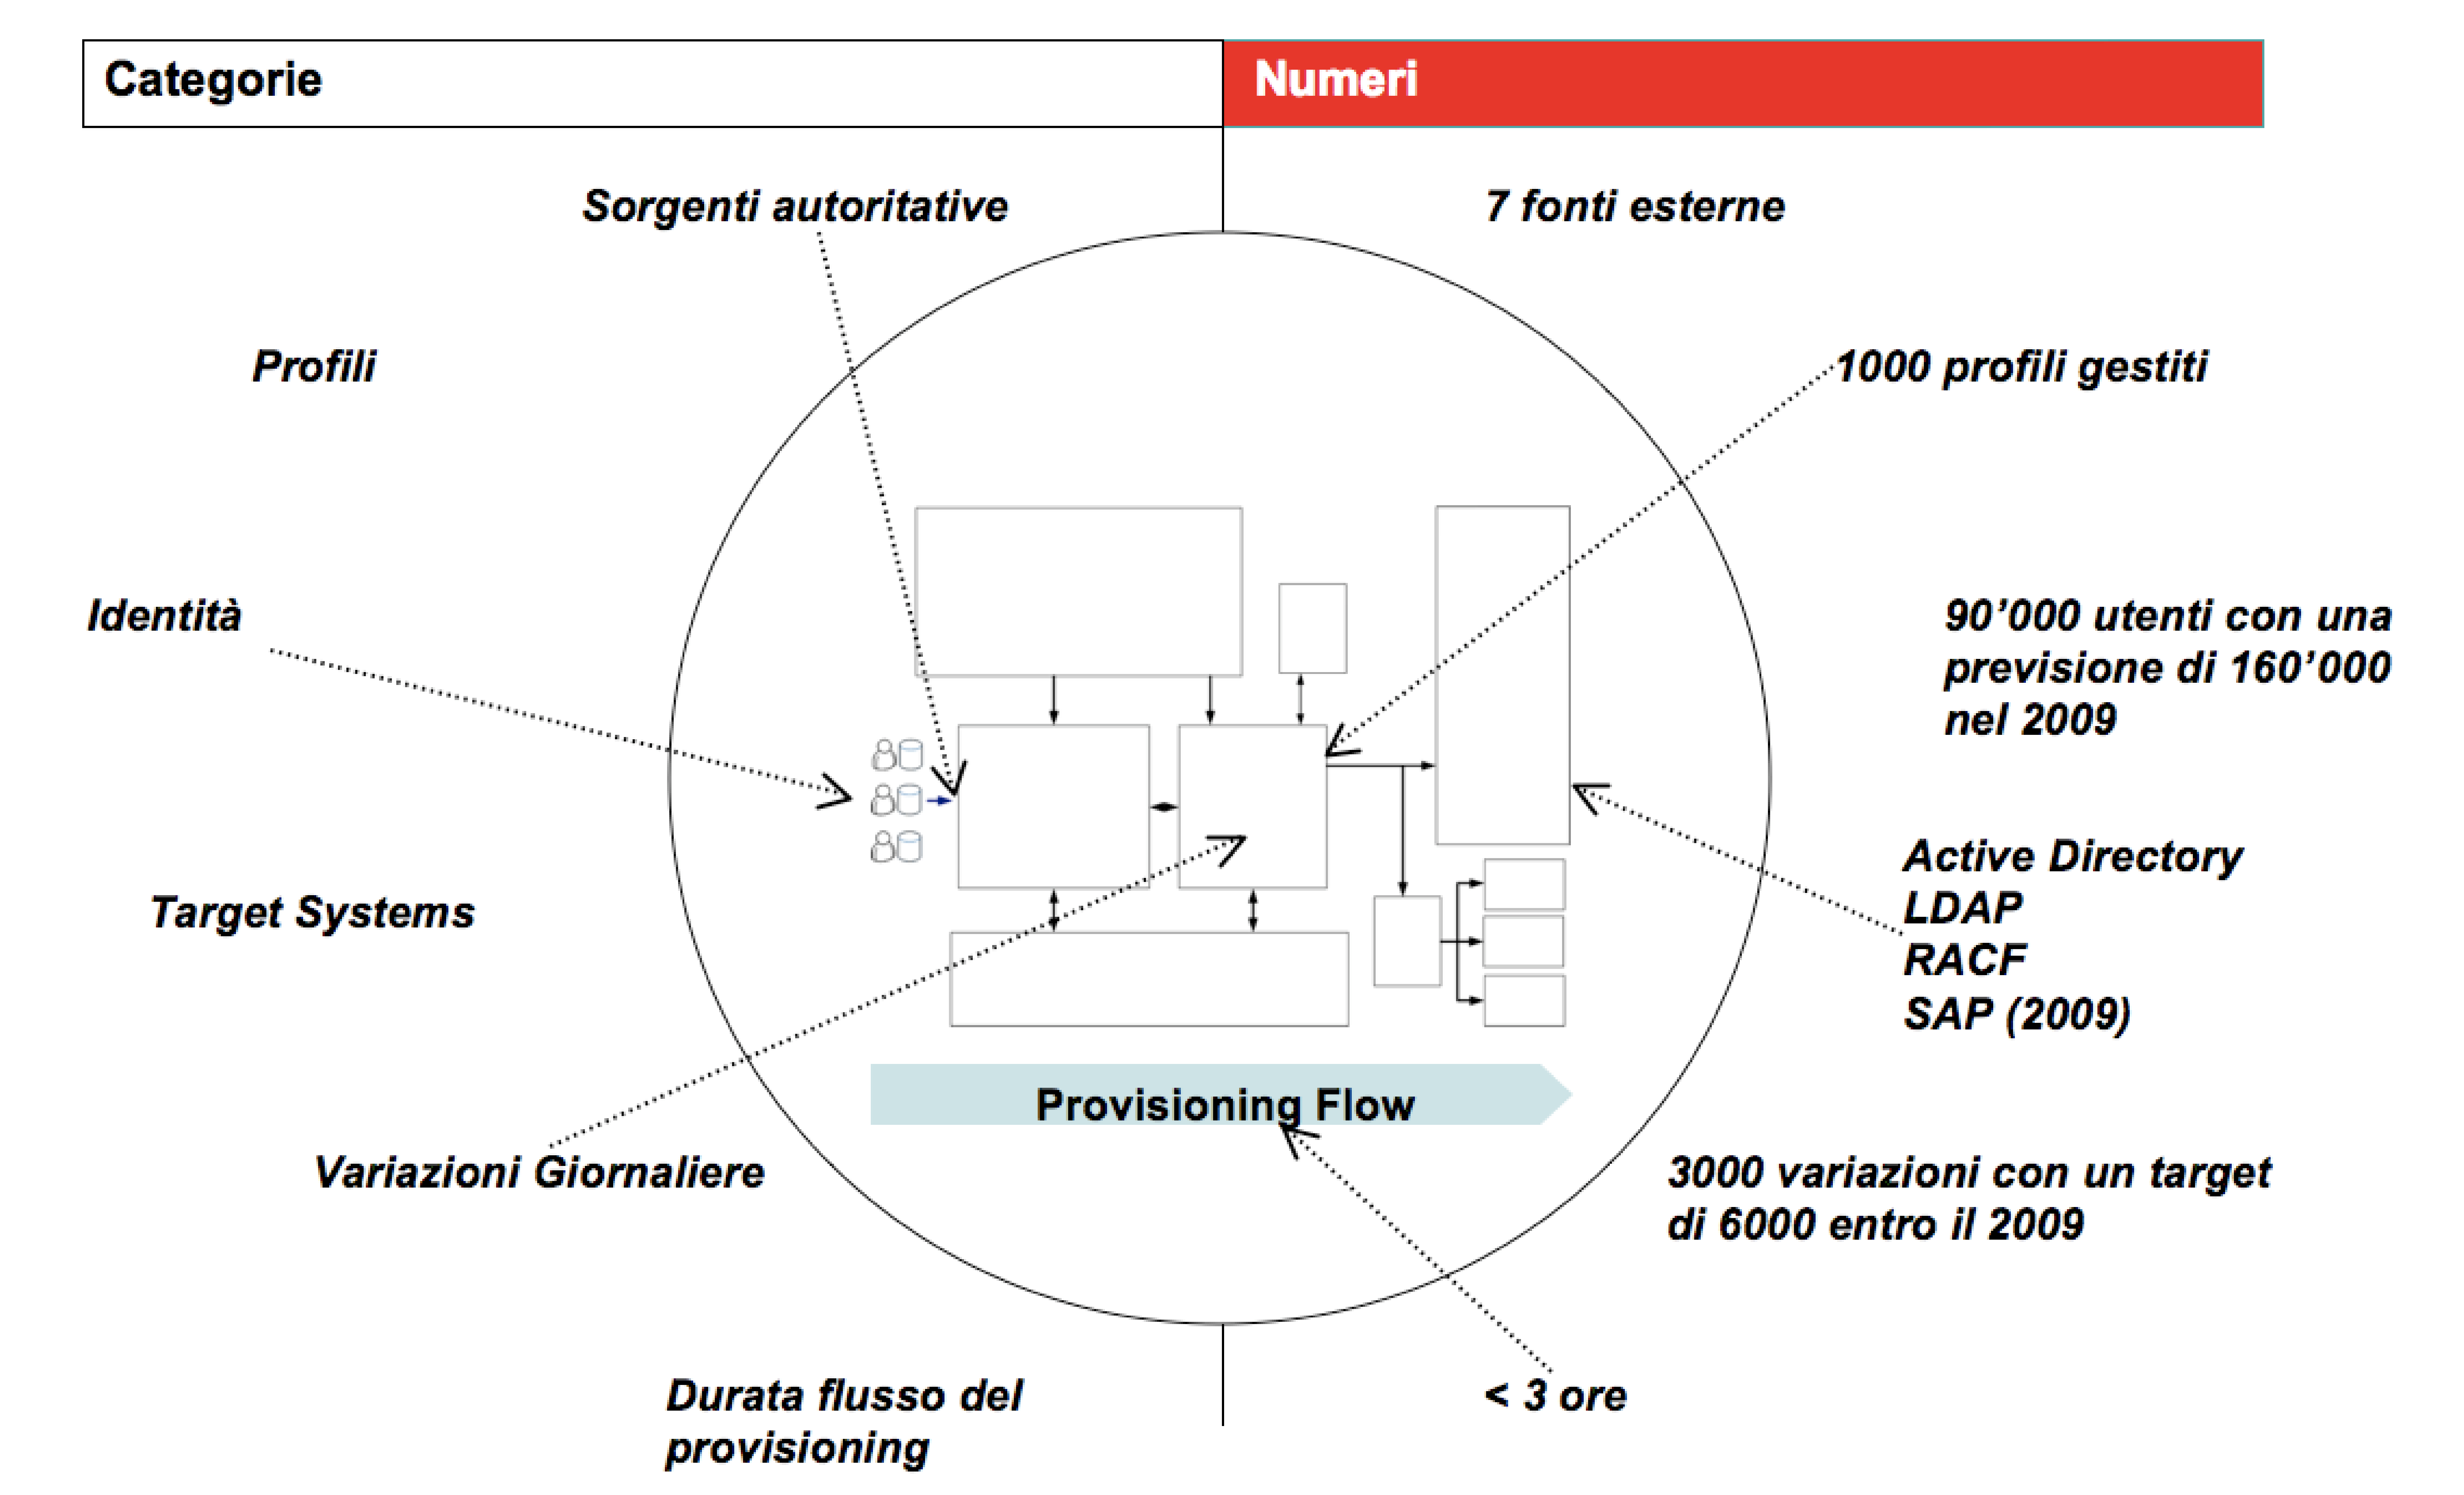
\includegraphics[width=0.95\textwidth]{img/descrizioneprogetto.eps}
\caption{Ordine di grandezza dei dati trattati}
\label{descrizioneprogetto}
\end{sidewaysfigure}

La gestione delle utenze avviene a partire da quanto presente nei data base
degli uffici del personale (HR). 
L'ufficio HR inserisce per ogni dipendente un profilo contenente tutte le
informazioni necessarie in base alle policy della singola azienda in un data
base. Normalmente i DB utilizzati sono ospitati su mainframe e principalmente
sono di tipo DB2~\cite{DB2}, anche se alcune fonti usano SQL server
2005~\cite{SQLServer2005} e perfino flat file.
Le basi di dati vengono denominate \textit{fonti autoritative}, per evidenziarne
il ruolo chiave che questi dati rivestono ai fini della definizione del profilo utente. 
La soluzione implementata comporta il minor impatto possibile sulla struttura
già presente in tutte le realtà che compongono il gruppo finanziario, nella
totalità dei casi ci si limita a leggere i dati forniti senza apportare alcuna
modifica alla sorgente.
I dati letti dalle sorgenti vengono elaborati dal nucleo del sistema di IAM,
componente che è stato reingenierizzato durante lo stage di laurea, e vengono
generate delle istruzioni di modifica del profilo utente in relazione alla
situazione consolidata dell'esecuzione precedente. Queste istruzioni comportano
delle sequenze di comandi sui profili degli utenti, che consistono in operazioni
di cancellazione, modifica o aggiunta di attributi. 
Le istruzioni e il meccanismo di modifica del profilo verrà trattato
approfonditamente nel seguito della relazione.
Il sistema target di tutte le azioni di modifica è un directory LDAP~\cite{LDAP}
che contiene un sottoalbero per ogni utente del sistema, la modifica di un
attributo comporta una serie di operazioni che vengono portate a termine sui
server in produzione, configurando l'immagine di ogni utente come richiesto dal
sistema di IAM.
La scelta di avere un server LDAP come interfaccia tra lo IAM e i sistemi target
è molto utile perchè permette di rendere indipendenti i due ambienti. Alla luce
di questa decisione implementativa è risultato facile sostituire il blocco
dell'ETL custom precedentemente in essere con una soluzione diversa senza
rompere l'equilibrio degli altri componenti dell'architettura.

Il nucleo del framework di IAM è composto da tre macro-componenti che
svolgono, ciascuna, una parte delle elaborazioni necessarie per portare a
termine in modo efficace ed efficiente l’interno processo di provisioning delle
identità e di gestione degli accessi:

\begin{itemize}
\item \textbf{ETL}: la componente di ETL (Extract, Transform, Load) si occupa
dell’estrazione, trasformazione e caricamento dei dati in un sistema di sintesi.
I dati vengono estratti da sorgenti quali database transazionali (DB2, SQL
Server), comuni file di testo (presenti in locale o prelevati da sistemi remoti)
o da altri sistemi informatici che forniscono le informazioni raccolte dai
sistemi di HR (Human Resource).
I dati prelevati subiscono quindi un processo di trasformazione, che consente ad
esempio di selezionare solo quelli che sono di interesse per il sistema,
normalizzare i dati, derivare nuovi parametri, cercare correlazioni tra
dati recuperati da differenti tabelle, etc.
Tale trasformazione ha lo scopo di rendere omogenei dati provenienti da sorgenti
diverse e di fare in modo che siano più aderenti alla logica di business del
sistema per cui viene sviluppato il processo di provisioning. 
L’ultima operazione svolta dalla componente ETL è quella di determinare le
variazioni presenti sui profili normalizzati rispetto alla situazione presente
in Admin e consolidata in precedenza. 

\item \textbf{Transaction}: la componente di Transaction ha il compito di prelevare le
informazioni generate dal modulo ETL e di procedere con l’aggiornamento dei profili
utente presenti in Admin applicando le trasformazioni indicate, così da
allineare il profilo utente su Admin con la situazione fornita dai sistemi di
HR.

\item \textbf{Admin}: eTrust Admin è una soluzione robusta e scalabile per il
provisioning di utenti tra molteplici ed eterogenei sistemi (Active
Directory, LDAP, RACF, etc.). Questo meccanismo consente, attraverso una corretta
configurazione di policy, la creazione, la modifica o la rimozione degli utenti
e dei relative oggetti sui diversi sistemi di un organizzazione.
Il vantaggio offerto da questa soluzione è che astrae i sistemi target,
presentando le principali caratteristiche in formato LDAP.
\end{itemize}
  
Mentre l’ultima componente, eTrust Admin, è un prodotto commerciale di
Computer Associates installato e configurato in modo appropriato, le prime due
sono frutto di attività di analisi, progettazione e implementazione svolte
appositamente per l’ambiente presente in azienda.

La parte di cui mi sono occupato principalmente riguarda il modulo di
ETL perché è la parte che più rappresentava un problema in termini di
prestazioni e scalabilità di tutta l'architettura esistente.
Quella che segue è una disamina dettagliata del processo eseguito da ETL e
Transaction, ovvero dalle due componenti custom dell’infrastruttura IAM in
questione.  

\subsection{Soluzione precedente}
Il modulo ETL è stato implementato con del codice custom, realizzato da un
gruppo di programmatori Java e progettato per lavorare strettamente con eTrust
admin attraverso l'interfacciamento LDAP.
Lo stato del sistema target era mantenuto mediante l'ausilio di un database di
appoggio di tipo INGRES~\cite{ingres}, in cui era memorizzato un record per ogni
utente e un hash che identificasse lo stato di ogni riga.
Lo pseudocodice è presentato nel listato~\ref{codicejava}, e descrive le
operazioni di elaborazione effettuate per ogni fonte autoritativa.

\begin{algorithm}
%\dontprintsemicolon

Connessione alla fonte autoritativa\;

\While{esistono utenti non elaborati}{
    Estrai tutte le informazioni presenti\;
    Normalizza il profilo rispetto al consolidato \;
    Applica le policy e ricava i privilegi \;
    Calcola Hash \;
    \If{Hash != Hash consolidato}
    {
        ModificaProfiloLDAP(ProfiloUtente)\;
        \If{Modifica\_riuscita}{
	ConsolidaProfilo \;
	}
    }
}
\label{codicejava}
\caption{Soluzione di ETL precedente}
\end{algorithm}

La trasformazione così implementata presenta diversi punti deboli e
inefficienze, che si è cercato di risolvere con la nuova implementazione:

\begin{enumerate}
\item La soluzione non è scalabile
\item Il codice è difficilmente riutilizzabile, vista la diversa natura delle
sorgenti
\item Non c'è una correlazione forte tra quanto presente nel directory di admin
e l'immagine consolidata dell'utente
\item Il codice è difficilmente manutenibile perchè la curva di apprendimento è
troppo ripida
\item Non è possibile dividere il calcolo delle modifiche e l'esecuzioni delle
operazioni in fasi distinte
\item Eventuali errori di acquisizione dei dati possono portare a modifiche
massive e indesiderate dei profili utente
\item \'E prevista solo un'esecuzione di tipo batch notturna, quando i dati non
vengono modificati
\end{enumerate}

Il raddoppio della base di utenza è stato il motivo principale che ha spinto il
passaggio dal meccanismo sopra descritto a uno più flessibile, che garantisse
degli standard di scalabilità e manutenibilità in linea con il resto
dell'architettura di IAM. 
Un altro punto debole significativo è la resistenza a errori nei dati in
ingresso. Potrebbe potenzialmente capitare (ed è capitato) che delle mancanze di
dati nelle sorgenti scatenassero processi di rimozione massiva indesiderata di
profili utente dai sistemi target, comportando fastidiosi disservizi.

\section{Nuova implementazione del modulo ETL}

Come introdotto poco sopra, il compito della componente di ETL è quello di
prelevare i dati provenienti da HR sotto forme e da sorgenti diverse per poi
procedere con la loro normalizzazione, il completamento degli stessi con
informazioni prelevate da tabelle aggiuntive, la rilevazione delle modifiche
sui profili utente e la generazione dell’input necessario alla Transaction per
allineare, su Admin, i profili degli utenti rilevati come modificati.   
Tutte queste operazioni devono essere fatte rispettando dei vincoli di tempo e
in modo parallelo, riducendo al minimo (possibilmenete eliminando) gli svantaggi
dell'architettura precedentemente in essere.

Lo strumento scelto come base di tutto l'ETL è SQL Server Integration
Services~\cite{SSIS}, che consiste in un modulo integrato in Visual Studio per
elaborare dati provenienti da data base.
Il prodotto in questione risulta essere molto comodo perchè permette agilmente
di:

\begin{itemize}
\item Trattare sorgenti eterogenee (file, DB2, fogli excel, SQL server) in modo
omogeneo
\item Lavorare in modo visuale sui dati 
\item Utilizzare il linguaggio SQL (Transaction-SQL) quando necessario
\item Compiere elaborazioni complesse usando dei linguaggi di programmazione
(Vb.net, VBS)
\end{itemize}

A parte la propaganda commerciale che, si sa, spesso lascia il tempo che trova,
SSIS si è dimostrato essere uno strumento robusto e affidabile, che ha davvero
reso facile l'implementazione della logica applicativa.
Lavorare sui dati ingresso sempre sotto forma di tuple e con gli strumenti
tipici del data mining ha permesso inoltre di avere delle performance molto
buone in termini di tempo di elaborazione e soprattutto ha permesso di mantenere
il codice dell'applicazione spesso immediato da capire.

In figura\ref{nuovaimplementazione} si può vedere lo schema logico di lavoro
della nuova implementazione del modulo ETL. 

\begin{figure}[htbp]
\centering
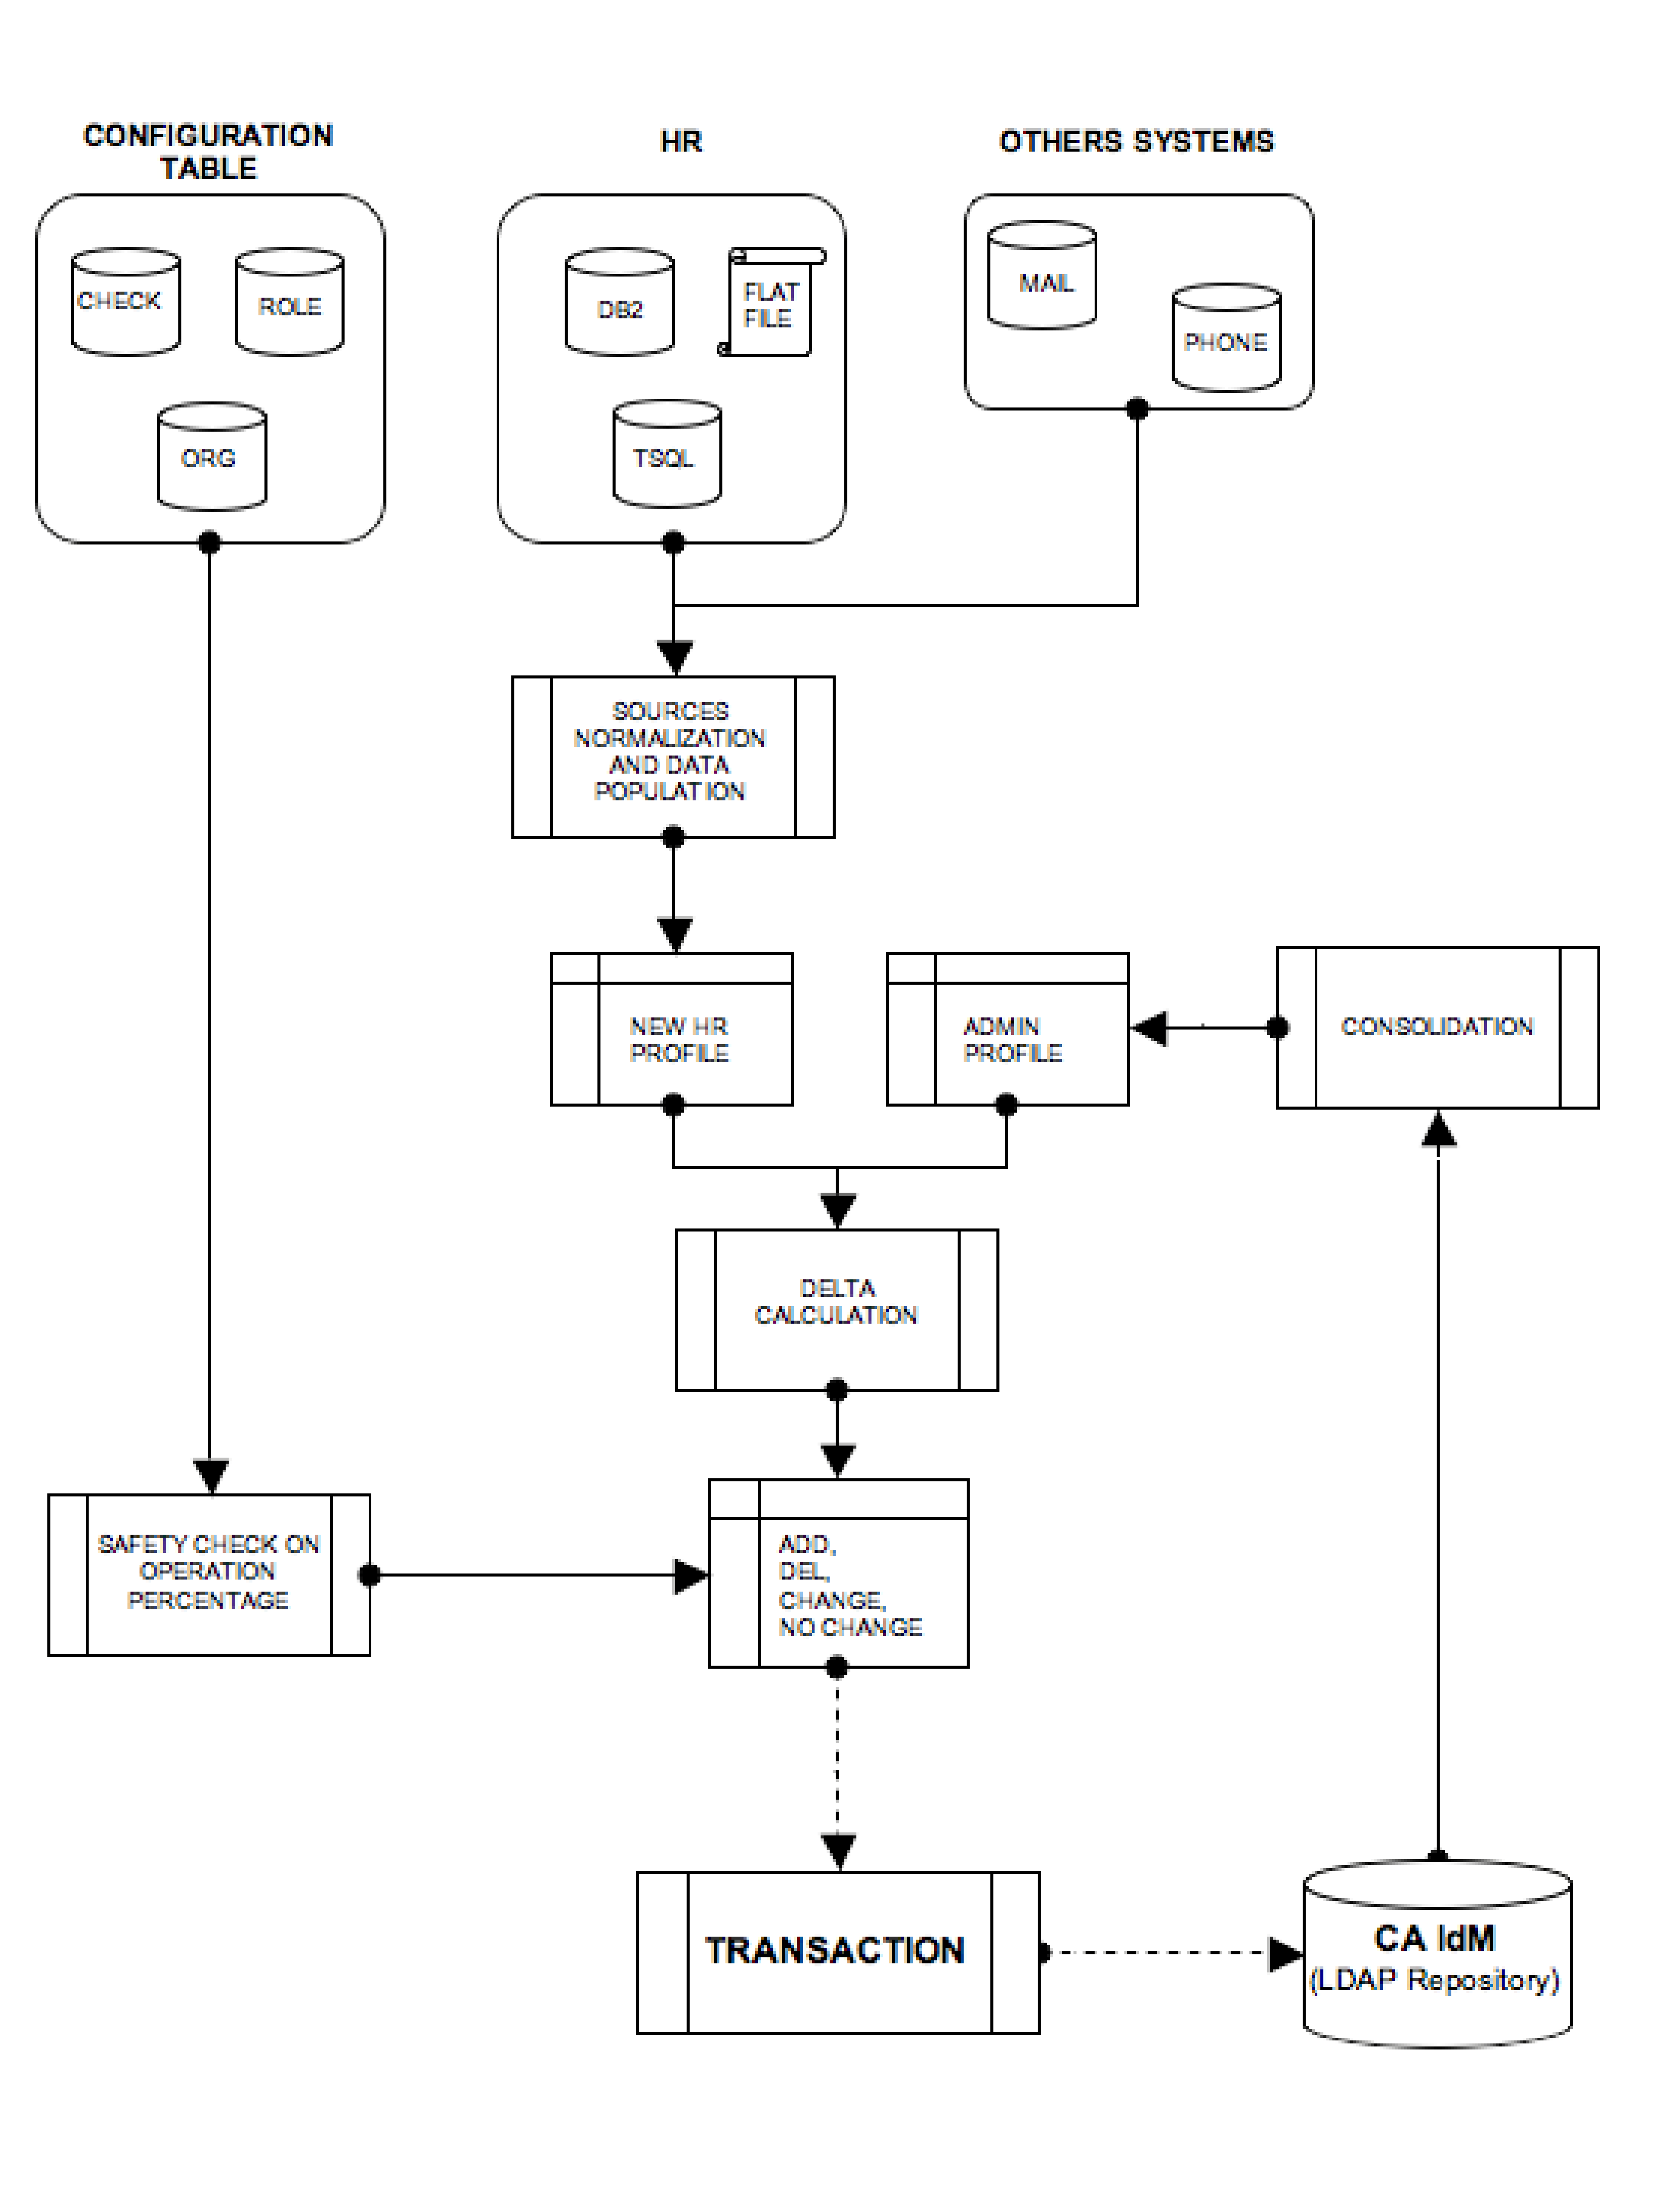
\includegraphics[width=0.95\textwidth]{img/nuovaimplementazione.eps}
\caption{Flusso logico ETL}
\label{nuovaimplementazione}
\end{figure}


\subsection{Concorrenza nell'accesso ai dati}
\subsection{Scalabilità}


% vim: tw=80 syntax=tex
